% Drawing 74/07-12 -- folder 74, batch 07, archive page 134 (PDF page 135).
% Transcription: un cube raturé ; un prisme surmonté d'une pyramide, avec les points $a', a, a''$ et $b', b, b''$ ; à droite une figure analogue développée ; une longue flèche vers le mot « bicarré ».
% Kind: prism with pyramid (two versions), long strokes. Method 2 (schematic redraw from the facsimile). Status: partial.
% Notes: A prism surmounted by a pyramid: the upper version (a box with two inner verticals, the roof from its apex to the two upper corners and a short stroke down from the apex), and below it the version with the apex s, the roof points a', a, a'' and the foot points b', b, b'' (the roof edges from s to a' and a'', the vertical from s through a down to b, the box a' a'' b'' b'); long strokes running to the right towards « u bicarré » (text, kept as in the issue-73 redraw). Every edge between the same vertex points. Struck out and omitted: the struck cube above (scribbled over). Still differs: the analogous developed figure at the right lies at the bbox edge and is only begun on the page there, so it is not drawn; the small prism sketch at the top left belongs to the heading « Prismes triangulaires » and is not drawn; the faint roof strokes from s towards b' and b'' are left out. Redrawn 2026-11-09 (issue 128): to check again.
% Coordinates: 1 unit = 1 mm = 1/100 of the crop width (bbox in page fractions: [0.1, 0.08, 0.65, 0.34]).
% Redrawn by Claude (claude-opus-5-5), issue #73, 2026-11-09; not checked by a human; not compiled (no TeX in the session).
% Rights: reproduces part of the work -- behind RENDER_TRANSCRIPTS, never published by itself.
\documentclass[tikz,border=3pt]{standalone}
\usepackage{amsmath,amssymb}
\usetikzlibrary{patterns,arrows.meta}
\tikzset{pencil/.style={black!45}, struck/.style={black!35}, mark/.style={circle,draw,inner sep=1.3pt}, pt/.style={circle,fill,inner sep=0.9pt}, opt/.style={circle,draw,fill=white,inner sep=1.1pt}}
\begin{document}
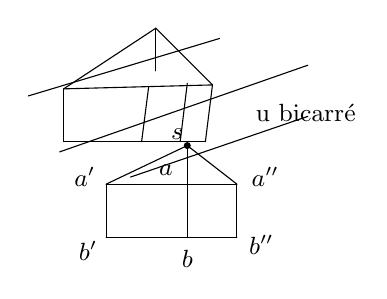
\begin{tikzpicture}[x=1mm,y=1mm,line cap=round,line join=round,font=\scriptsize]
\draw (29,-42) -- (47.9,-41.5);
\draw (47.9,-41.5) -- (47,-48.7);
\draw (47,-48.7) -- (29,-48.7);
\draw (29,-48.7) -- (29,-42);
\draw (40.7,-34.3) -- (29,-42);
\draw (40.7,-34.3) -- (47.9,-41.5);
\draw (34.4,-54.1) -- (51,-54.1);
\draw (34.4,-54.1) -- (34.4,-60.9);
\draw (51,-54.1) -- (51,-60.9);
\draw (34.4,-60.9) -- (51,-60.9);
\draw (44.7,-49.2) -- (34.4,-54.1);
\draw (44.7,-49.2) -- (51,-54.1);
\draw (44.7,-49.2) -- (44.7,-54.1);
\draw (44.7,-54.1) -- (44.7,-60.9);
\draw (40.7,-34.3) -- (40.7,-39.7);
\draw (39.8,-41.7) -- (38.9,-48.7);
\draw (44.7,-41.3) -- (43.8,-48.7);
\node[pt] at (44.7,-49.2) {};
\draw (24.5,-42.9) -- (48.8,-35.6);
\draw (28.5,-50) -- (60,-39);
\draw (37.5,-53.2) -- (60,-45.5);
\node[inner sep=1pt] at (43.4,-47.8) {\small $s$};
\node[inner sep=1pt] at (31.7,-53.2) {\small $a'$};
\node[inner sep=1pt] at (42,-52.3) {\small $a$};
\node[inner sep=1pt] at (54.6,-53.2) {\small $a''$};
\node[inner sep=1pt] at (32.1,-62.6) {\small $b'$};
\node[inner sep=1pt] at (44.7,-63.6) {\small $b$};
\node[inner sep=1pt] at (54.1,-61.8) {\small $b''$};
\node[inner sep=1pt,anchor=west] at (53,-45) {\small u bicarré};
\end{tikzpicture}
\end{document}
